\section{Evaluation and Discussion}

We evaluate all the described implementations on real-world RDFs.
We measure the full time of query execution including all overhead on data preparation.
This way we can estimate the applicability of the matrix-based algorithm to real-world problems.

For evaluation, we use a PC with Ubuntu 18.04 installed.
It has Intel core i7-6700 CPU, 3.4GHz, DDR4 64Gb RAM, and Geforce GTX 1070 GPGPU with 8Gb RAM.

\subsection{Dataset}
As far as it was shown that matrix-based CFPQ algorithms are performant enought to handle big RDF~\cite{Mishin:2019:ECP:3327964.3328503}, we extend CFPQ\_Data dataset~\cite{Mishin:2019:ECP:3327964.3328503} with new RDFs: \textit{go-hierarchy, go, enzime, core, pathways, eclass-514en}, and use the extended dataset in our evaluation. Also we add Geospecies RDF and related query from~\cite{Kuijpers:2019:ESC:3335783.3335791}. 
Detailed description of th dataset and queries are provided in appendix~\ref{section:dataset}.


\subsection{Evaluation Results}
We provide results only for a part of the collected dataset because of the page limit.
Running time is measured in seconds, RAM memory consumption is measured in megabytes unless specified otherwise.

The results of the CFPQ evaluation are presented in tables \ref{tbl:tableRDFQ1}, \ref{tbl:tableRDFQ2} and \ref{tbl:tableGeospeciesResults}.
We can see that the running time of both CPU and GPGPU versions for the relational query semantics is small even for graphs with a big number of vertices and edges.
The relatively small number of edges of interest may be the reason for such behavior.
We believe it is necessary to extend the dataset with new queries which involve more different types of edges.
Also, we can see, that $\textbf{RG\_CUSP}_{\textit{rel}}$ implementation which uses CUSP requires more memory.

As we can see, the matrix-based algorithm for relational query semantics implemented for RedisGraph is more than 1000 times faster than the one based on annotated grammar implemented for Neo4j~\cite{Kuijpers:2019:ESC:3335783.3335791} and uses more than 4 times less memory.
We can conclude that the matrix-based algorithm is more performant than other CFPQ algorithms for query evaluation under a relational semantics for real-world data processing.

Also, we can see, that the GPGPU version which utilizes sparse matrices is significantly faster than the other implementations especially on big graphs. For example, for Geospacies it more than 7 times faster in both relational and single-path scenarios.
Note, that for GPGPU versions we include time required for data transferring and formats convertion.

We can conclude, that the cost of computing matrices with PathIndexes for single-path query semantics is not high. On average, it is about 2 times slower than the reachability matrix calculation. The additional running time of the path extraction is presented in figure~\ref{fig:extractTime}. As we can see, this time is small and linear in length of the path.

Finally, we conclude that the matrix-based algorithm paired with a suitable database and employing appropriate libraries for linear algebra is a promising way to make CFPQ with relational and single-path query semantics applicable for real-world data analysis.
We show that SuiteSparse-based CPU implementation is performant enough to be comparable with GPGPU-based implementations on real-world data.



{\setlength{\tabcolsep}{0.4em}
\begin{table*}[h]
\caption{RDFs query $G_1$}
\label{tbl:tableRDFQ1}
\rowcolors{3}{}{lightgray}
\begin{tabular}{| l | c  c | c  c | c  c | c  c | c  c |}
    \hline

    \multirow{3}{*}{Name}   &   \multicolumn{6}{|c|}{Relational semantics index}	&	\multicolumn{4}{|c|}{Single path semantics index} \\
    \cline{2-11}
    	    &	\multicolumn{2}{|c|}{RG\_CPU\textsubscript{rel}}	&	\multicolumn{2}{|c|}{RG\_CUSP\textsubscript{rel}}	&	\multicolumn{2}{|c|}{RG\_SPARSE\textsubscript{rel}} &	\multicolumn{2}{|c|}{RG\_CPU\textsubscript{path}}	&	\multicolumn{2}{|c|}{RG\_SPARSE\textsubscript{path}}	 \\
    \cline{2-11}
            &   Time & Mem &  Time     & Mem & Time     & Mem  &  Time     & Mem & Time     & Mem \\
    \hline
    \hline
    atom-primitive              & 0.016 & 1.2  & 0.016 & 0.1 & 0.005 & 0.1  & 0.033 & 1.5  & 0.008 & 0.1  \\
biomedical-mesure-primitive & 0.016 & 0.6  & 0.012 & 0.1 & 0.005 & 0.1      & 0.027 & 1.3  & 0.007 & 0.1  \\
core                        & 0.004 & 0.3  & 0.022 & 2   & 0.01  & 0.1      & 0.002 & 0.3  & 0.016 & 0.1  \\
eclass\_514en                 & 0.067 & 13.8 & 0.075 & 14  & 0.166 & 16     & 0.195 & 31.2 & 0.496 & 26   \\
enzyme                      & 0.018 & 5.9  & 0.021 & 0.1 & 0.018 & 4        & 0.029 & 8.1  & 0.043 & 6    \\
foaf                        & 0.002 & 0.4  & 0.013 & 0.1 & 0.006 & 0.1      & 0.024 & 0.4  & 0.009 & 0.1  \\
funding                     & 0.006 & 0.5  & 0.019 & 0.1 & 0.006 & 0.1      & 0.057 & 0.5  & 0.009 & 0.1  \\
generations                 & 0.002 & 0.3  & 0.01  & 0.1 & 0.004 & 0.1      & 0.013 & 0.3  & 0.005 & 0.1  \\
go-hierarchy                & 0.091 & 16.3 & 0.433 & 650 & 0.108 & 121.2    & 0.976 & 92   & 0.336 & 125  \\
go                          & 0.604 & 28.8 & 0.59  & 70  & 0.365 & 30.2     & 1.286 & 75.7 & 0.739 & 45.4 \\
pathways                    & 0.011 & 0.1  & 0.019 & 0.1 & 0.007 & 0.1      & 0.021 & 0.5  & 0.021 & 2    \\
people\_pets                & 0.017 & 0.4  & 0.025 & 0.1 & 0.007 & 0.1      & 0.031 & 0.6  & 0.011 & 0.1  \\
pizza                       & 0.03  & 1.8  & 0.021 & 4   & 0.006 & 0.1      & 0.075 & 5.5  & 0.009 & 0.1  \\
skos                        & 0.001 & 0.1  & 0.008 & 0.1 & 0.004 & 0.1      & 0.005 & 0.3  & 0.006 & 0.1  \\
travel                      & 0.004 & 0.3  & 0.022 & 2   & 0.007 & 0.1      & 0.008 & 0.3  & 0.01  & 0.1  \\
univ-bench                  & 0.002 & 0.3  & 0.01  & 0.1 & 0.005 & 0.1      & 0.013 & 0.3  & 0.007 & 0.1  \\
wine                        & 0.017 & 3.5  & 0.032 & 6   & 0.009 & 0.1      & 0.117 & 7.1  & 0.015 & 0.2  \\
    \hline
  \end{tabular}
\end{table*}
}


{\setlength{\tabcolsep}{2pt}
\begin{table}[h]
\caption{Geospecies querying results}
\label{tbl:tableGeospeciesResults}
\rowcolors{3}{}{lightgray}
\begin{tabular}{| c  c | c  c | c  c | c  c |}
    \hline

    \multicolumn{4}{|c|}{Relational semantics index}	&	\multicolumn{4}{|c|}{Single path semantics index} \\

    \hline


    \multicolumn{2}{|c|}{RG\_CPU\textsubscript{rel}}	&	\multicolumn{2}{|c|}{RG\_SPARSE\textsubscript{rel}} & \multicolumn{2}{|c|}{RG\_CPU\textsubscript{path}}	&	\multicolumn{2}{|c|}{RG\_SPARSE\textsubscript{path}}	 \\
    \hline
    Time & Mem & Time & Mem & Time & Mem & Time & Mem \\
    \hline
    \hline
    7.146 & 16934.2 & 0.856 & 5274 & 15.134 & 35803.6 & 1.935 & 5282   \\
    \hline
  \end{tabular}
\end{table}
}


\begin{figure*}
\begin{subfigure}{0.32\textwidth}
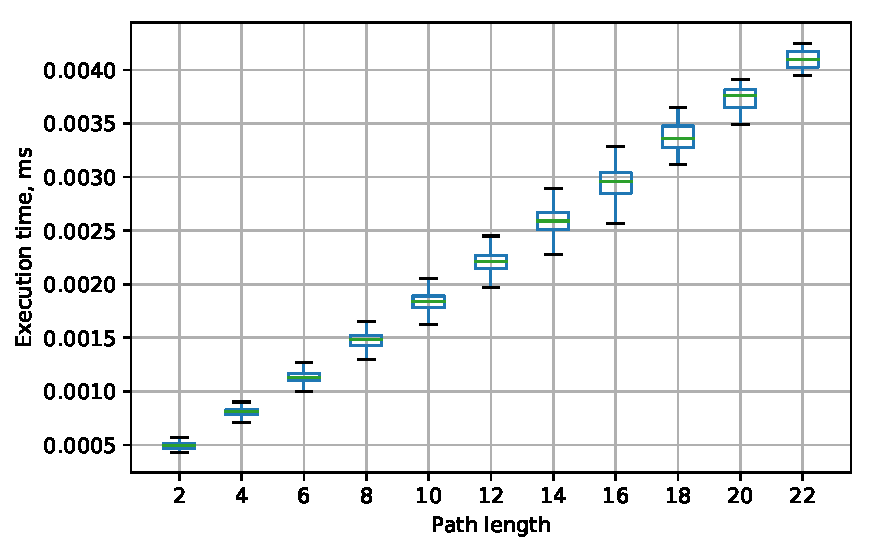
\includegraphics[width=\linewidth,trim=0 0 -1.5cm 0]{plots/G1_go.pdf}
\caption{$go$ and $G_1$} \label{fig:extractTimeGoG1}
\end{subfigure}
\hspace*{\fill} % separation between the subfigures
\begin{subfigure}{0.32\textwidth}
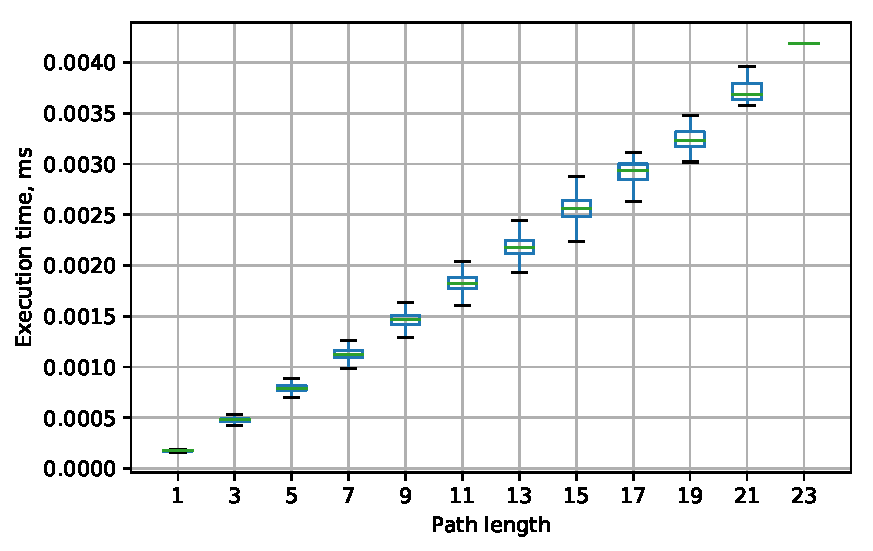
\includegraphics[width=\linewidth,trim=0 0 -1.5cm 0]{plots/G2_go.pdf}
\caption{$go$ and $G_2$} \label{fig:extractTimeGoG2}
\end{subfigure}
\hspace*{\fill} % separation between the subfigures
\begin{subfigure}{0.32\textwidth}
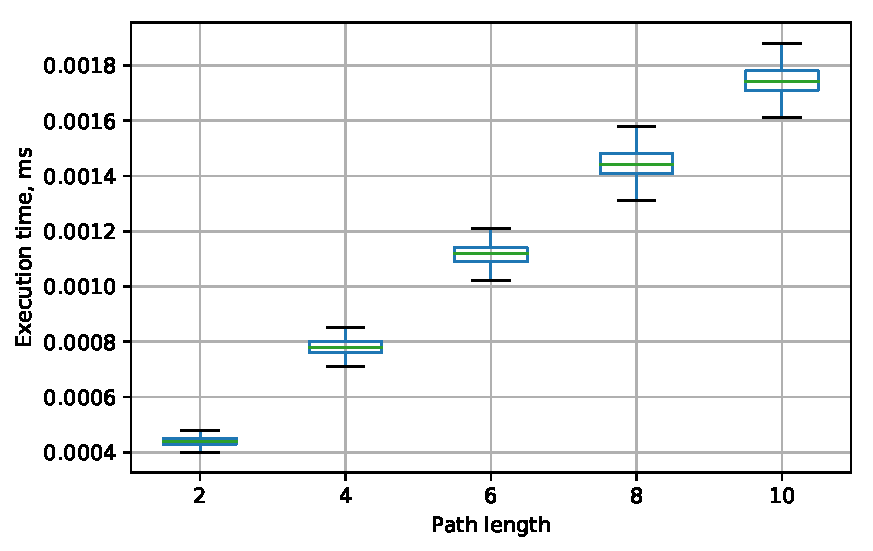
\includegraphics[width=\linewidth,trim=0 0 -1.5cm 0]{plots/Geo_geospicies.pdf}
\caption{$geospicies$ and $geo$} \label{fig:extractTimeGeo}
\end{subfigure}
\caption{Execution time of the path extraction algorithm depending on the path length}
\label{fig:extractTime}
\end{figure*}

